\chapter{Implementation}
\label{chap:Implementation}

\section{Broker Implementation}
\label{sec:Broker Implementation}

A system-block diagram, showing the interactions between the various gamq
submodules, can be seen in Figure~\ref{fig:systemBlockDiagram}.

\subsection{Connection Manager}
\label{sub:connectionManager}

As mentioned in Section~\ref{sec:codestructure}, the Connection Manager has two
main functions, accepting incomming connections, and parsing incomming arguments
in compliance with the protocol (Section~\ref{sec:protocol}).

The acceptance of incomming connections requires the specifics of each protocol
(\gls{tcp}/\gls{udp}/\gls{http} etc.) to be abstracted away using a standard
interface through which messages can be sent to clients, the 'writer' interface
in this case. An example of the UDP writer interface can be seen in
Appendix~\ref{appendix:udpWriter}. Once connected, each client is serviced by a
seperate GoRoutine in an \emph{Event Loop}-style pattern - the main Connection
Manager thread performs the minimal amount of work necessary before farming a
client out to a background thread, in order to prevent one connecting client
from blocking another.

The parsing of each client message is simply a matter of tokenisation and
pattern matching, as seen in Appendix~\ref{appendix:parseClientCommand}. The
biggest performance gains to be exploited in a message broker are in ensuring
efficient serialization and deserialization of messages - so this was a focus of
the protocol parsing logic, as explored in Section~\ref{sub:performance}.

\todo[inline]{Overview of the connection manager (TCP/UDP connections etc.)}

\subsection{Message Storage}
\label{sub:messageStorage}

In the event that, for whatever reason, a client is not ready to accept a
message when it arrives - this message must be buffered up in a datastructure of
some kind, until delivery is possible. There are a number of different
datastructures that could be used - each with its own pros and cons. \\

As mentioned in Section~\ref{sub:pubsub}, message brokers typically support a
number of different delivery patterns, the two most common of which are Queues
(Section~\ref{sub:queues}) and Topics (Section~\ref{sub:topics}). The backing
datastructures used for each are explored below. \\

Queues require that messages are delivered in the order they are pushed onto the
queue, and that each message is delivered to a single consumer - so any backing
datastructure must support this. Queues typically support two main operations:

\begin{description}
  \item[\textit{enqueue(m)}] \hfill \\
    The message $m$ is placed onto the queue.
  \item[\textit{dequeue()}] \hfill \\
    Returns the message at the front of the queue (optionally blocks whilst the queue is empty)
\end{description}

The simplest method of representing a queue of messages, would be an array. New
messages are inserted into the first unoccupied slot in the array, and messages
are read front-to-back, in a \gls{fifo} fashion.

\begin{figure}[H]
  \centering
  \begin{subfigure}[b]{\textwidth}
    \centering
    \begin{tikzpicture}

\coordinate (s) at (0,0);
\foreach \num in {0,...,6}{
    \ifthenelse{\num < 4}
    {\node[draw, minimum size=1cm] at (s) (\num) {m\num};} % Fill the box
    {\node[draw, minimum size=1cm] at (s) (\num) {};} % Don't fill the box

    \coordinate (s) at ($(s) + (1,0)$);
}

\node[above=1mm of 0] {$h$};
\node[above=1mm of 4] {$t$};

\end{tikzpicture}

    \caption{Messages are read from the head of the queue ($h$)}
    \label{fig:tikz:queueArrayInitial}
  \end{subfigure}

  \begin{subfigure}[b]{\textwidth}
    \centering
    \begin{tikzpicture}

\coordinate (s) at (0,0);
\foreach \num in {0,...,6}{
    \ifthenelse{\num > 0 \AND \num < 4}
    {\node[draw, minimum size=1cm] at (s) (\num) {m\num};} % Fill the box
    {\node[draw, minimum size=1cm] at (s) (\num) {};} % Don't fill the box

    \coordinate (s) at ($(s) + (1,0)$);
}

\node[above=1mm of 0] {$h$};
\node[above=1mm of 4] {$t$};

\end{tikzpicture}

    \caption{The array is shuffled down}
    \label{fig:tikz:queueArrayHeadRead}
  \end{subfigure}

  \begin{subfigure}[b]{\textwidth}
    \centering
    \begin{tikzpicture}

\coordinate (s) at (0,0);
\foreach \num in {1,...,7}{
    \ifthenelse{\num < 4}
    {\node[draw, minimum size=1cm] at (s) (\num) {m\num};} % Fill the box
    {\node[draw, minimum size=1cm] at (s) (\num) {};} % Don't fill the box

    \coordinate (s) at ($(s) + (1,0)$);
}

\node[above=1mm of 1] {$h$};
\node[above=1mm of 4] {$t$};

\end{tikzpicture}

    \caption{The next message is now ready to be read}
    \label{fig:tikz:queueArrayPostShuffle}
  \end{subfigure}
  \caption{Reading a message from an array-based queue}
  \label{fig:tikz:queueArray}
\end{figure}

However, there are several disadvantages of this approach, for both the enqueue and dequeue operations.

\begin{description}
  \item[\textit{enqueue(m)}] \hfill \\
    Arrays in GoLang have a fixed length - but there is no limit on the number
    of messages a queue may be asked to buffer. We can compensate for this by
    using 'slices' instead of arrays\todo{Explain slices - seperate section} -
    which are expandable using the \mintinline{go}{append()} command
    (Listing~\ref{lst:golangAppendToSlice}). The message $m$ is stored into the
    first available array index, which will typically complete in $O(1)$ time.
    However, in order to create the illusion of an 'expandable' array, slices
    use a fixed-length array under the hood - which is expanded when full. This
    expansion involves creating a new array, which is twice the size of the
    original. Each message in the underlying array is then copied to the new
    array, which is used for all slice actions going forward. Therefore, whilst
    the vast majority of messages will be stored in $O(1)$ time, a message that
    triggers an expansion of the underlying array will require $O(n)$ time to
    store (where $n$ is the number of messages in the queue)\todo{Improve
    notation}.
  \item[\textit{dequeue()}] \hfill \\
    Pulling the first message in the array requires that the array be shuffled
    after each \mintinline{go}{dequeue()} operation, so that the next message to
    be delivered always resides in  array position 0 (see in
    Figure~\ref{fig:tikz:queueArray}). An array implementation would be
    extremely inefficient, requiring $n - 1$ items to moved down an array
    position. However, because a slice is simply a 'view' onto an array, this
    operation can be made extremely efficient - by simply creating a new slice,
    with all but the first element in common with the original.\todo{Diagram?}
    It is therefore possible to complete this operation in $O(1)$ time.
\end{description}

\begin{listing}[H]
  \centering
  \RecustomVerbatimEnvironment{Verbatim}{BVerbatim}{}
  \inputminted[firstline=7, lastline=12]{go}{code/snippets/appendToSlice.go}
  \caption{An example of appending to a GoLang slice}
  \label{lst:golangAppendToSlice}
\end{listing}

In addition to the disadvantages given above, slices are quite inefficient when
it comes to memory utilisation. At any moment in time, up to 50\% of the
underlying array will be empty. Whilst these array indexes do not contain
messages, they still occupy space in memory, meaning that (in the worst case
scenario) $O(2n)$ space is required to store $n$ messages. This is not ideal.

An alternative method of representing an in-memory-queue, is a linked list
(Figure~\ref{fig:tikz:queueLinkedList}). This has numerous advantages over an
array - with both enqueue and dequeue operations completing in $O(1)$ time.
Linked lists also improve on the space complexity of the queue, as the
datastructure grows and shrinks in response  to the number of messages - meaning
that we require $O(n)$ memory to store $n$ messages.

\begin{description}
  \item[\textit{enqueue(m)}] \hfill \\
    The item at the tail of the queue ($t$) - seen in
    Figure~\ref{fig:tikz:queueLinkedListInitial} - is simply updated with a
    pointer to $m$. This is an $O(1)$ operation, and simple to perform.
  \item[\textit{dequeue()}] \hfill \\
    The item at the head of the queue ($h$) is returned. The head pointer is
    then updated to point to the next message to be read, as in
    Figure~\ref{fig:tikz:queueLinkedListHeadRead}.
\end{description}

\begin{figure}[H]
  \centering
  \begin{subfigure}[b]{\textwidth}
    \centering
    \begin{tikzpicture}[thick]

\coordinate (s) at (0,0);
\foreach \num[remember=\num as \previous] in {0,...,4}{
    \node[draw, minimum size=1cm] at (s) (\num) {m\num};

    \ifthenelse{\num > 0}
    {\draw[->](\previous) edge (\num);}
    {}

    \coordinate (s) at ($(s) + (2,0)$);
}


\node[above=0.5cm of 0] (head) {$h$};
\node[above=1mm of 4] {$t$};
\draw[->,thick](head) edge (0);

\end{tikzpicture}

    \caption{Messages are read from the head of the queue ($h$)}
    \label{fig:tikz:queueLinkedListInitial}
  \end{subfigure}

  \begin{subfigure}[b]{\textwidth}
    \centering
    \begin{tikzpicture}[thick]

\coordinate (s) at (0,0);
\foreach \num[remember=\num as \previous] in {0,...,4}{
    \ifthenelse{\num < 2}
    {\node[draw, minimum size=1cm, gray] at (s) (\num) {m\num};}
    {\node[draw, minimum size=1cm] at (s) (\num) {m\num};}

    \ifthenelse{\num < 3}
    {\ifthenelse{\num > 0}{\draw[->, gray](\previous) edge (\num);}{}}
    {\draw[->](\previous) edge (\num);}

    \coordinate (s) at ($(s) + (2,0)$);
}


\node[above=0.5cm of 2] (head) {$h$};
\node[above=1mm of 4] {$t$};
\draw[->](head) edge (2);

\end{tikzpicture}

    \caption{Head moves, and read nodes are marked for garbage collection}
    \label{fig:tikz:queueLinkedListHeadRead}
  \end{subfigure}

  \begin{subfigure}[b]{\textwidth}
    \centering
    \begin{tikzpicture}[thick]

\coordinate (s) at (0,0);
\foreach \num[remember=\num as \previous] in {0,...,4}{
    \ifthenelse{\num < 2}
    { % These have been garbage collected
      \node[draw, minimum size=1cm, gray] at (s) (\num) {m\num};
      \node(Cross) [draw,cross out,minimum width=1cm,minimum height=1cm,red] at (s) {};
    }
    { % These are still active
      \node[draw, minimum size=1cm] at (s) (\num) {m\num};
    }

    % Don't draw 'next' pointers for dead nodes
    \ifthenelse{\num > 2}{\draw[->](\previous) edge (\num);}{}

    \coordinate (s) at ($(s) + (2,0)$);
}

\node[above=0.5cm of 2] (head) {$h$};
\node[above=1mm of 4] {$t$};
\draw[->](head) edge (2);

\end{tikzpicture}

    \caption{At some point in the future (depending on memory pressure), the
             \gls{gc} will automatically clean up the read messages}
    \label{fig:tikz:queueLinkedListGCRun}
  \end{subfigure}
  \caption{Reading a message from an array-based queue}
  \label{fig:tikz:queueLinkedList}
\end{figure}

A full implementation of a linked list queue can be found in
Appendix~\ref{appendix:queueCode}.

When it comes to representing topics, the situation is similar. As mentioned in
Section~\ref{sub:topics}, the main difference between queues and topics, is the
fact that queues deliver each message to a single consumer, whereas topics
deliver each message to \emph{all} consumers. This requires a subtly different
datastructure to hold the messages - as consumers may read messages at different
rates. If we use an array-based datastructure, similar to that in
Figure~\ref{fig:tikz:queueArray}, we would be required to maintain a seperate
queue for each subscriber to read from - as shown in
Figure~\ref{fig:tikz:arrayTopic}. A topic with $s$ subscribers, and $n$ pending
messages would therefore require at \emph{least} $O(n * s)$ memory, and that is
without considering the caveats described above\todo{??}. \\

\begin{figure}[H]
  \centering
  \begin{tikzpicture}[thick]

\coordinate (s) at (0,0);
\coordinate (t) at (0,-2);
\coordinate (u) at (0,-4);

\foreach \num in {0,...,6}{
    \ifthenelse{\num < 4}
    {\node[draw, minimum size=1cm] at (s) (1-\num) {m\num};} % Fill the box
    {\node[draw, minimum size=1cm] at (s) (1-\num) {};} % Don't fill the box

    \coordinate (s) at ($(s) + (1,0)$);
}

\foreach \num in {1,...,7}{
    \ifthenelse{\num < 4}
    {\node[draw, minimum size=1cm] at (t) (2-\num) {m\num};} % Fill the box
    {\node[draw, minimum size=1cm] at (t) (2-\num) {};} % Don't fill the box

    \coordinate (t) at ($(t) + (1,0)$);
}

\foreach \num in {0,...,6}{
    \ifthenelse{\num < 4}
    {\node[draw, minimum size=1cm] at (u) (3-\num) {m\num};} % Fill the box
    {\node[draw, minimum size=1cm] at (u) (3-\num) {};} % Don't fill the box

    \coordinate (u) at ($(u) + (1,0)$);
}

\node[above=1mm of 1-0] {$h$};
\node[above=1mm of 1-4] {$t$};

\node[above=1mm of 2-1] {$h$};
\node[above=1mm of 2-4] {$t$};

\node[above=1mm of 3-0] {$h$};
\node[above=1mm of 3-5] {$t$};

\node[left=1cm of 1-0] (s1) {Subscriber1 Messages};
\node[left=1cm of 2-1] (s2) {Subscriber2 Messages};
\node[left=1cm of 3-0] (s3) {Subscriber3 Messages};

  \draw[->] (1-0) edge (s1);
  \draw[->] (2-1) edge (s2);
  \draw[->] (3-0) edge (s3);

\end{tikzpicture}

  \caption{An array implementation of a topic}
  \label{fig:tikz:arrayTopic}
\end{figure}

A linked-list implementation, however, has the potential to be highly efficient
when it comes to storage space. Rather than storing $s$ messages, we can simply
keep multiple 'head' pointers on the same linked-list, one for each subscriber.
When a subscriber consumes a message - only the head pointer belonging to it is
moved up the list, the rest remain static
(Figure~\ref{fig:tikz:linkedListTopic}). Similar to the queue implementation,
the \gls{gc} will dispose of messages once all consumers have read them (all of
the 'subscriber' pointers have passed that message in the chain -
Figure~\ref{fig:tikz:queueLinkedList}). This method only requires $O(s + m)$
memory, for a topic with $s$ subscribers, and $m$ messages. The linked-list
implementation of a topic therefore has an even bigger efficiency saving over
the corresponding array-based implementation, than in the queue examples given
above, as seen in Figure~\ref{fig:tikz:implementationSpaceComplexityGraph}.

\begin{figure}[H]
  \centering
  \begin{tikzpicture}[thick]

\coordinate (s) at (0,0);
\foreach \num[remember=\num as \previous] in {0,...,4}{
    \node[draw, minimum size=1cm] at (s) (\num) {m\num};

    \ifthenelse{\num > 0}
    {\draw[->](\previous) edge (\num);}
    {}

    \coordinate (s) at ($(s) + (2,0)$);
}


\node[above=0.5cm of 0] (s1) {$s1$};
\node[above=0.5cm of 1] (s2) {$s2$};
\node[below=0.5cm of 0] (s3) {$s3$};

\node[above=1mm of 4] {$t$};
\draw[->,thick](s1) edge (0);
\draw[->,thick](s2) edge (1);
\draw[->,thick](s3) edge (0);

\end{tikzpicture}

  \caption{A linked-list implementation of a topic}
  \label{fig:tikz:linkedListTopic}
\end{figure}

\begin{figure}[H]
  \centering
  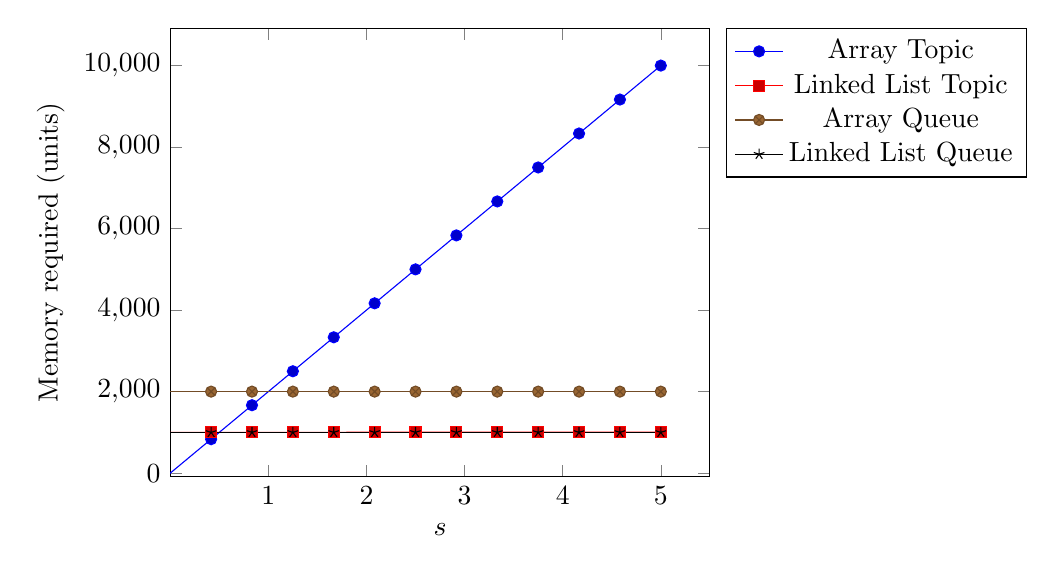
\begin{tikzpicture}
\begin{axis}[
    xlabel=$s$,
    ylabel={Memory required (units)},
    xmin=0,
    xtick={1,...,10},
    scaled ticks=false,
    legend entries={Array Topic, Linked List Topic, Array Queue, Linked List Queue},
    legend pos=outer north east,
]
\addplot {2 * x * 1000};
\addplot {x + 1000};
\addplot {2 * 1000};
\addplot {1000};
\end{axis}
\end{tikzpicture}

  \caption{A comparison of the space complexities of various queue/topic
           implementations, as the number of subscribers ($s$) increases}
  \label{fig:tikz:implementationSpaceComplexityGraph}
\end{figure}

\subsection{Message Shipper}
\label{sub:Message Shipper}

The Message Shipper is responsible for pulling messages off an internal gamq
queue/topic (Section~\ref{sub:messageStorage}), and sending them to consumers.
Thanks to the blocking characteristic of GoChannels
(Section~\ref{sub:golangConcurrency}), this is as simple as listening to the
GoChannel attached to the subscribers queue/topic, encoding messages as they are
pulled off the queue and sending the bytes to the 'writer' object created by
the Connection Manager (Section~\ref{sub:connectionManager}) - as seen in
Appendix~\ref{appendix:sendMessagesToClient}.

\subsection{Metrics Manager}
\label{sub:Metrics Manager}

As shown in Figure~\ref{fig:systemBlockDiagram}, all other blocks in the system
produce performance metrics, to be formatted as StatsD
(Section~\ref{sub:StatsD}) messages, for graphing and visualisation. These
metrics are aggregated by the Metrics Manager, before being sent to InfluxDB
(Section~\ref{sub:InfluxDB}). Whilst important, sending metrics should never
impact the performance of the broker itself - so the metrics manager uses a
'\emph{buffered GoChannel}'\cite{channelsInGo}. Unlike a normal GoChannel,
putting a message on a buffered channel will not block in the event that the
GoRoutine on the other end is not currently listening\footnote{Assuming the
buffer is not full}. Once the Metrics Manager has received a metric from the
channel, it adds the value to a local buffer - which it flushes once a second,
formatting all buffered metrics as lightweight StatsD UDP packets
(Section~\ref{sub:StatsD}) - which it sends to the configured StatsD network
address (Section\ref{sec:Configuration}).

\section{Presentation Interface}
\label{sec:presentationInterface}

\subsection{StatsD}
\label{sub:StatsD}

StatsD is an open-source statistics daemon, written by developers at
\href{https://www.etsy.com/uk/}{Etsy} in 2010\cite{statsd}, and which has seen
widespread adoption by infrastructure teams ever since. The project aims to
define a simple protocol (Listing~\ref{lst:statsdSchema}) for sending statistics
over the network, and to make it simple to aggregate and store those metrics for
real-time analysis. StatsD can differentiate between metrics of different types:

\begin{listing}
  \centering
  \mintinline{text}{metricname:1|c}
  \caption{A simple counter metric, exactly as it would appear inside a network packet}
  \label{lst:statsdSchema}
\end{listing}

\begin{description}
  \item[Counters] A simple counter that can be incremented or decremented. An
  example use case could be the number of messages sent through a broker.
  \item[Timing] The amount of time taken to complete a task. An example could be
  the amount of time taken to process a message.
  \item[Gauges] An arbitrary value, stored until it is superseded by a new
  value. An example of this could be the number of connections open to the
  broker at a single point in time.
\end{description}

These packets can be sent over the network as either TCP or UDP packets. Packets
can contain multiple metrics, separated with newline characters
(Listing~\ref{lst:statsdMultiplePackets}), which can greatly improve the
efficiency of the transfer, as the size of each metric (the order of a few
bytes) is far below the maximum capacity of a single packet - whilst the typical
\gls{mtu} of Ethernet networks is ~1500 bytes\cite{rfc1191}. Gamq uses the UDP
protocol by default (although this is configurable, see
Section~\ref{sec:Configuration} for details), as the cost of sending UDP packets
is very low cost when compared to TCP, and we do not require the deliverability
guarantees of TCP (metrics are non-critical). Metrics are typically sent over a
\gls{lan}, where packet loss is usually quite low. In the event that is it not,
but the packet loss is uniform, the loss of some metrics should not affect the
overall trend of the data too adversely.

\begin{listing}
  \centering
  \mintinline{text}{gorets:1|c\nglork:320|ms\ngaugor:333|g\nuniques:765|s}
  \caption{Multiple metrics in a single packet}
  \label{lst:statsdMultiplePackets}
\end{listing}

\subsection{InfluxDB}
\label{sub:InfluxDB}

InfluxDB is an open-source, NoSQL database, optimised for the storage and
retrieval of \gls{time-series data}. Influx is part of a family of databases
designed to store (amongst other things) a large amount of metrics data at very
high speed (the order of millions of events per second), which also includes
\href{http://graphite.wikidot.com/}{Graphite} and
\href{http://opentsdb.net/}{OpenTSDB}. InfluxDB was chosen for this project due
to its maturity (compared to OpenTSDB) and performance (compared to
Graphite/Carbon).

\subsection{Grafana}
\label{sub:Grafana}

\begin{figure}[H]
  \centering
  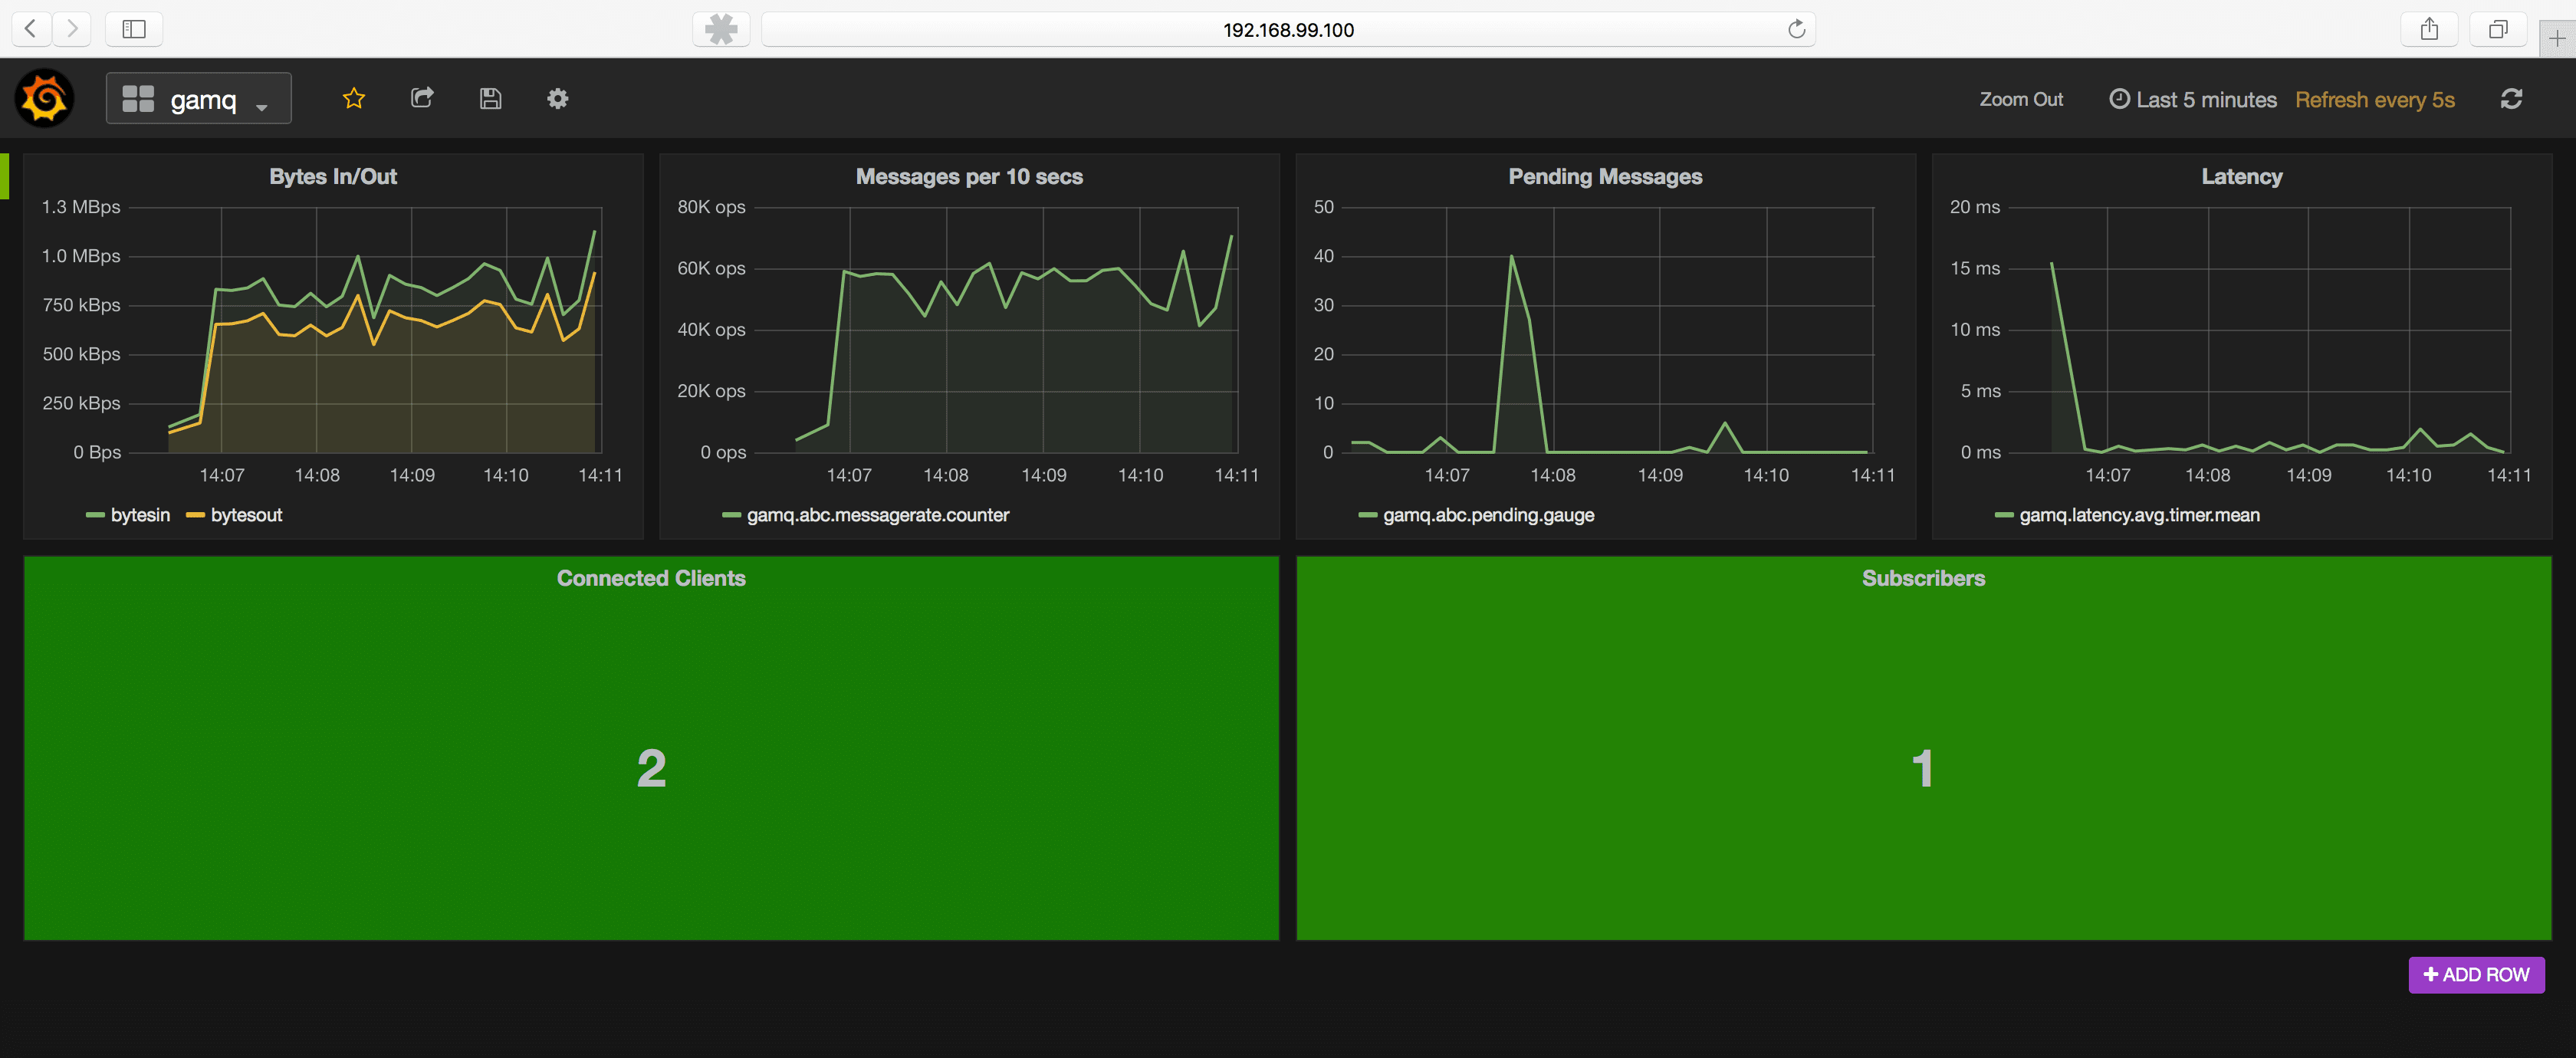
\includegraphics[width=0.8\textwidth]{figures/grafanaMidBenchmark}
  \caption{A screenshot of the Grafana visualisation tool}
  \label{fig:grafanaMidBenchmark}
\end{figure}

\href{http://grafana.org/}{Grafana} is an open-source visualisation tool for
\gls{time-series data}, typically that which is produced by Internet
infrastructure and application analytics. Developed by a consortium of Internet
companies as a modern replacement for the previously popular
\href{https://github.com/graphite-project/graphite-web}{Graphite-Web} project.
Grafana can visualise \gls{time-series data} from a variety of data-sources,
such as the ElasticSearch, the aforementioned Graphite and, most importantly,
InfluxDB.

\subsection{Docker}
\label{sub:dockerDesign}

As mentioned in Section~\ref{sub:StatsD}, gamq is designed to send StatsD
messages (Section~\ref{sub:StatsD}) across the network. In a production
environment, these would be sent to the above software stack, running on a
separate server in the datacenter. In a development environment, the metrics
stack could be run on a development server, or the developers local machine. The
configured monitoring stack should therefore be as portable as possible, to make
development as simple as possible. \href{https://www.docker.com/}{Docker} allows
environments to be defined in code, and built into container images - which can
be run in a manner similar to that of a lightweight virtual machine. The Docker
container gamq sends metrics to is available
\href{https://github.com/FireEater64/docker-statsd-influxdb-grafana}{on Github}.
